\hypertarget{tulokset}{%
\chapter{Tulokset}\label{tulokset}}

\hypertarget{prototyyppiohjelman-esittely}{%
\section{Prototyyppiohjelman
esittely}\label{prototyyppiohjelman-esittely}}

Prototyyppiohjelma on yksinkertainen yhden sivun selainsovellus. Sen
avulla voi luoda käyntejä, laskuttaa niitä, koota laskuja
koontilaskuiksi ja hyvittää yksittäisiä laskurivejä.

Ohjelman pääkäyttöliittymä on esitetty kuvassa
\ref{rakkine_default-view}

Laskujen sisältöjä voi tarkastella, ja ohjelma laskee laskujen avoimet
summat.

Lisäksi käyttöliittymästä voi valita maksajan luotavalle laskulle.
Mikäli maksajia valitaan useampia, ohjelma jakaa käynnit kahdelle eri
maksajalle. Tämä on esitetty kuvassa \ref{rakkine_dividing}

\begin{figure}
\centering
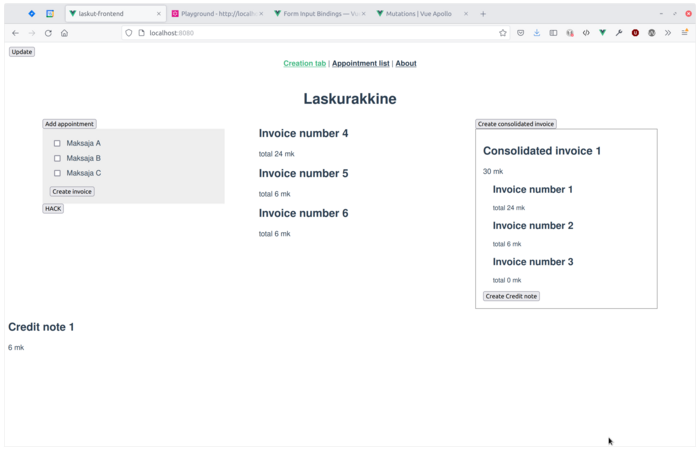
\includegraphics{illustration/screenshots/Laskurakkine.png}
\caption{\label{rakkine_default-view}Laskujen lisäysnäkymä}
\end{figure}

Erillisessä listanäkymässä (Kuva \ref{rakkine_list-view}) voi
tarkastella luotujen käyntien tilaa sekä laskutettavan myynnin tilaa.
Ohjelma näyttää, onko käynti laskutettu vai laskuttamaton. Myynnin
osalta ohjelma näyttää, miten myynti jakautuu eri maksajille, ja onko
summa avoin, laskutettu vai hyvitetty.

\begin{figure}
\centering
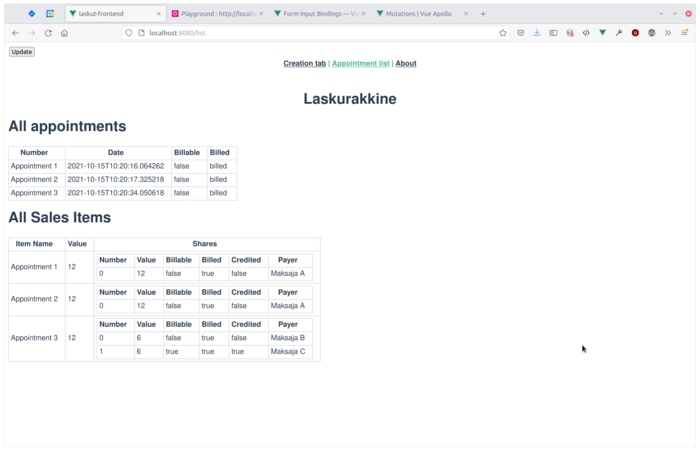
\includegraphics{illustration/screenshots/List-view.png}
\caption{\label{rakkine_list-view}Ohjelman listanäkymä}
\end{figure}

\begin{figure}
\centering
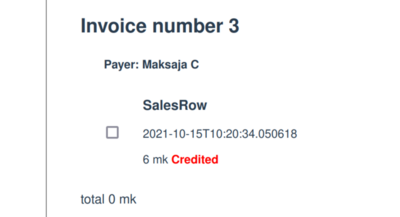
\includegraphics{illustration/screenshots/credited.png}
\caption{\label{rakkine_credited}Ohjelma näyttää, että yksittäinen
laskurivi on hyvitetty}
\end{figure}

Kuvassa \ref{rakkine_credited} on esitetty miten ohjelma näyttää
hyvitetyn laskurivin.

\begin{figure}
\centering
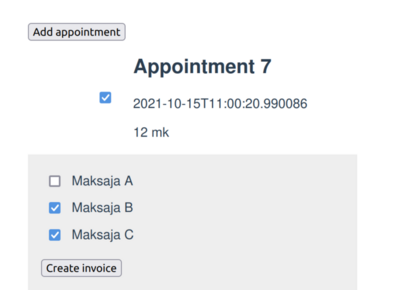
\includegraphics{illustration/screenshots/Dividing.png}
\caption{\label{rakkine_dividing}Esimerkki käynnin jakamiesta usealle
maksajalle}
\end{figure}

Käytin asiakasohjelman tekemiseen niin vähän aikaa kuin mahdollista. Se
näkyy tyylin hiomattomuutena. Luonnosmaisen näköinen ulkoasu myös
kommunikoi muille prosessiin osallistuville, että ohjelmisto tai
etenkään sen käyttöliittymä ei ole tarkoitettu tuotantokäyttöön, vaan
apuvälineeksi erilaisten tietomallin piirteiden kartoittamiseen.

\hypertarget{parannuksia-tietomalliin}{%
\section{Parannuksia tietomalliin}\label{parannuksia-tietomalliin}}

Viiden viikon aikana syntyi pieni malli laskutukseen tietorakenteen
parantamiseksi. Lisäksi löytyi kaksi pientä ideaa, joita voi hyödyntää,
kun ohjelmistoa kehitetään.

Pieni malli laskutuksen parantamiseksi on esitetty kuvassa
\ref{finalmodel1-again}. Se pitää sisällään ajatuksen käynnin
muuttumisesta myynniksi, kun se saapuu laskutuksen piiriin. Oma
erikoisuutensa on myös käynnin jakamiseen liittyvä jakoperuste - tätä ei
ohjelmistoon toteutettu, mutta suunnitteluvaiheessa se tuntui
hyödylliseltä idealta.

\begin{figure}
\centering
\includegraphics{illustration/malli4.jpg}
\caption{\label{finalmodel1-again}Lopullinen malli}
\end{figure}

Kaksi pientä ideaa ovat molemmat käyttökelpoisia erillään mallista.
Ensimmäinen niistä on myynnin, myyntirivin ja hyvitysrivin välinen
tiivis yhteysketju. Tämä idea (kuva \ref{finalidea1})mahdollistaa hyvin
yksinkertaisen ja joustavan myynnin laskutus- ja hyvityslogiikan.

\begin{figure}
\centering
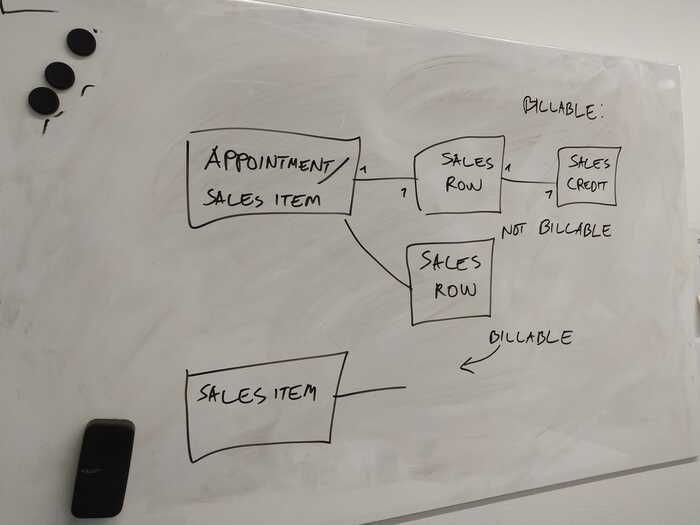
\includegraphics{illustration/final-idea-1.jpg}
\caption{\label{finalidea1}Idea 1}
\end{figure}

Toinen pieni idea on, että käynti kannattaisi erottaa selkeästi laskulle
tulevasta myynnistä. Tällöin on mahdollista myös esimerkiksi vaihtaa
myöhemmin maksajaa, jolta käynti laskutetaan, ilman että jo
muodostettuihin laskuihin tarvitsee kajota. Tämä ajatus on esitetty
kuvassa \ref{finalidea2}.

\begin{figure}
\centering
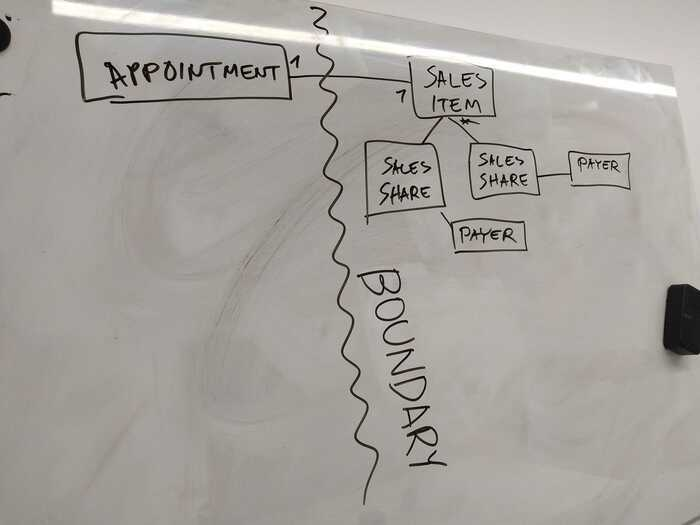
\includegraphics{illustration/final-idea-2.jpg}
\caption{\label{finalidea2}Idea 2}
\end{figure}
